\documentclass[colorBG,slideColor,8pt]{beamer}
\mode<presentation>
{
  % Use the IIS-theme
  \usetheme{FHL}
  % Der mathematische Schriftsatz ist mit Serifen
  \usefonttheme[onlymath]{serif}
  % Noch nicht aufgedeckte Punkte erscheinen ausgegraut
%  \setbeamercovered{transparent}
  % Bild-/Tabellenüberschriften sind sehr klein
  \setbeamerfont{caption}{size=\tiny}
}

\usepackage[ngerman]{babel}
\usepackage[utf8]{inputenc}
\usepackage{amsmath,bm}
\usepackage{accents}
\usepackage[]{easymovie}
\usepackage{lmodern}
\usepackage{helvet} 
\usepackage{setspace}
\renewcommand{\familydefault}{\sfdefault}

\usepackage{etoolbox}
\usepackage{booktabs}
\usepackage{tabulary}
\usepackage{multirow}

\usepackage[version-1-compatibility]{siunitx}
\sisetup{detect-family, locale=DE}

\usepackage{caption}
\captionsetup[figure]{name=}
\captionsetup[table]{name=}

\usepackage{subcaption}
\captionsetup[subfigure]{list=true, font=tiny, labelfont=bf, 
	labelformat=brace, position=bottom, singlelinecheck=off, justification=raggedright}

%
% Dick der Folientitel 1. Folie
%
\newcommand{\talktitle}{Evaluierung von Methoden zur Bestimmung der ventilatorischen Schwellen in der Spiroergometrie} 
%
% Some useful macros:
\newcommand{\MatDef}[2]{\left[ \hspace{-0.4em} \begin{array}{#1} #2 \end{array} \hspace{-0.4em} \right]}
\newcommand{\E}[1]{\ensuremath{\mathrm{E}\hspace{-0.12em}\left\{#1\right\}}}
\newcommand{\real}[1]{\ensuremath{\mathrm{Re}\hspace{-0.12em}\left\{#1\right\}}}
\newcommand{\imag}[1]{\ensuremath{\mathrm{Im}\hspace{-0.12em}\left\{#1\right\}}}
\newcommand{\ex}[1]{\ensuremath{e^{#1}}}
\newcommand{\rect}[1]{\ensuremath{\mathrm{rect}\left(#1\right)}}
\newcommand{\tri}[1]{\ensuremath{\mathrm{tri}\left(#1\right)}}
\newcommand{\mycos}[1]{\ensuremath{\cos{\left(#1\right)}}}
\newcommand{\mysin}[1]{\ensuremath{\sin{\left(#1\right)}}}
\newcommand{\corrbone}{\quad  \mbox{$\circ$  \hspace{-0.65em} --- \hspace{-0.65em}  $\bullet$}  \quad}
\newcommand{\invcorrbone}{\quad  \mbox{$\bullet$  \hspace{-0.65em} --- \hspace{-0.65em}  $\circ$}  \quad}
\newcommand{\maker}[1]{\textcolor{red!80!black}{#1}}
\newcommand{\makeg}[1]{\textcolor{green!74!black}{#1}}
\newcommand{\makeb}[1]{\textcolor{blue!80!black}{#1}}
\newcommand{\eqotwo}{EQO\textsubscript{2}}
\newcommand{\eqcotwo}{EQCO\textsubscript{2}}
\newcommand{\votwo}{\.{V}O\textsubscript{2}}
\newcommand{\vcotwo}{\.{V}CO\textsubscript{2}}
\newcommand{\ve}{\.{V}E}

% Literaturverzeichnis:
\usepackage[autostyle=true,german=quotes]{csquotes}
\usepackage[
backend=biber,
style=iso-authoryear,
autolang=other,
bibencoding=UTF8,
maxnames=3,
hyperref
]{biblatex}
\renewcommand*{\bibfont}{\scriptsize}
\DefineBibliographyStrings{ngerman}{andothers={et\ al\adddot}}
\addbibresource{Referenzen.bib}

\AtBeginSection[]{
		\frame{
		\frametitle{}
		\tableofcontents[currentsection]
		}
}

\apptocmd{\UrlBreaks}{\do\f\do\m}{}{}
\setcounter{biburllcpenalty}{9000}% Kleinbuchstaben
\setcounter{biburlucpenalty}{9000}% Großbuchstaben
%
% -----------------------------------------------------------
% Begin
% -----------------------------------------------------------
\begin{document}
% -----------------------------------------------------------
% Title page
% -----------------------------------------------------------
\begin{frame}
    \vspace{-10ex}
    \textcolor{fhlred}{\HRuleFill[0.4ex]} \\ \vspace{1ex}
    {\linespread{1.5}\selectfont
    \MakeUppercase{\bf \huge \talktitle}\\[5.5ex]}
    \normalsize Kolloquium zur Bachelorthesis\\
    \textcolor{fhlred}{\HRuleFill[0.1ex]} \\ \vspace{4ex}
    \small Julian-Marvin Lütten\\
    \small Fachhochschule Lübeck, B.Sc. Biomedizintechnik\\
    \vspace{2ex}
    \small angefertigt bei der\\
    \small cardioscan GmbH\\
    \small 2018
\end{frame}

\begin{frame}{Inhalt}
\tableofcontents
\end{frame}

% -----------------------------------------------------------
% Kapitel 1: Relevanz der Arbeit
% -----------------------------------------------------------

\section{Relevanz der Arbeit}

\begin{frame}{Trend der Fitness-Wirtschaft}
\begin{figure}[H]
	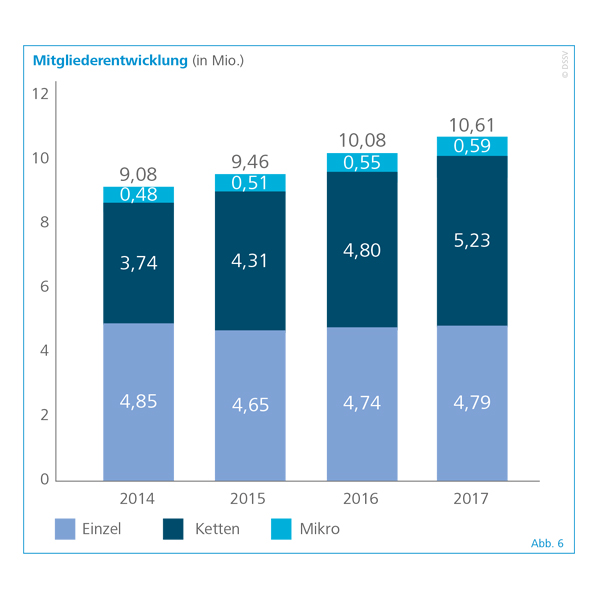
\includegraphics[width=5cm]{Bilder/Mitgliederentwicklung.png}
	\caption{Mitgliederentwicklung in dt. Fitnessstudios~(\cite{DSSV.2018})}
\end{figure}
\end{frame}

\begin{frame}{Spiroergometrie bei cardioscan}
\begin{itemize}
	\item cardioscan GmbH bietet u.a. Spiroergometrie-Systeme an
	\item Zweck: Definition von individuellen Trainingsbereichen
	\item Neues Spiroergometer \textsl{metabolicscan} soll künftige Hardware darstellen
	\item Forschungsstand: Detektion von Stoffwechselübergängen durch Bestimmung der ventilatorischen Schwellen~(\cite{Westhoff.2012})
	\item Vorheriger Software-Algorithmus: HF (VT2) $\hat{=}$  HF (RQ $=$ 1)\\$\rightarrow$ akut beeinflussbar $\rightarrow$ anfällig für Fehler und wissenschaftlich umstritten
	\item Vielzahl an möglichen Alternativen $\rightarrow$ Welche ist am besten geeignet?
\end{itemize}
\end{frame}

% -----------------------------------------------------------
% Kapitel 2: Das ventilatorische Schwellenkonzept
% -----------------------------------------------------------

\section{Das ventilatorische Schwellenkonzept}

\begin{frame}
\begin{itemize}
	\item Zunehmende körperliche Arbeit $\rightarrow$ steigender Energiebedarf $\rightarrow$ metabolische Reaktion: Stoffwechselumstellungen: aerob $\rightarrow$ aerob-anaerob $\rightarrow$ anaerob
	\item Erhöhte Glykolyse-Rate $\rightarrow$ Laktatproduktion $\rightarrow$ zusätzlich anfallendes CO\textsubscript{2} $\rightarrow$ messbare Zunahme der \vcotwo{} und \ve
	\item Prinzip: Respirationsmessung in festen Abständen $\rightarrow$ grafische Darstellung
	\item Bestimmung der ventilatorischen Schwellen mit jeweils zwei ausgewählten Methoden je Schwelle (\cite{Westhoff.2012})
\end{itemize}
\begin{columns}
\begin{column}{\linewidth}
\begin{figure}[H]
	\begin{subfigure}[t]{0.2\linewidth}
		\centering
		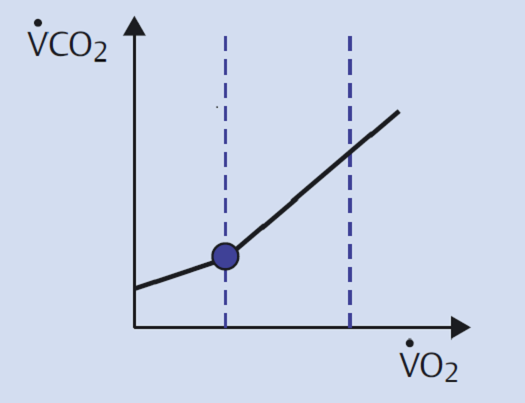
\includegraphics[width=\linewidth]{Bilder/vslope.png}
		\subcaption{V-Slope:\\überproportionaler Anstieg der \vcotwo}
	\end{subfigure}
	\hfil
	\begin{subfigure}[t]{0.2\linewidth}
		\centering
		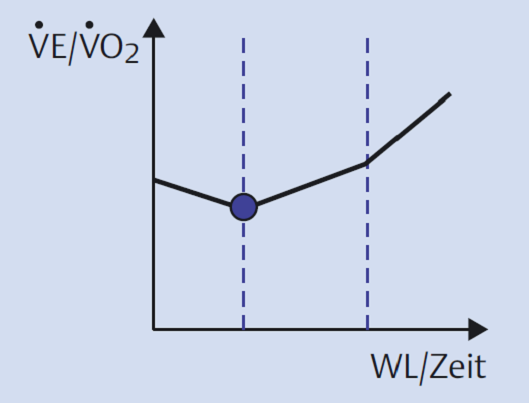
\includegraphics[width=\linewidth]{Bilder/eqo2.png}
		\subcaption{\eqotwo:\\Punkt des optimalen Wirkungsgrades}
	\end{subfigure}
	\hfil
	\begin{subfigure}[t]{0.2\linewidth}
		\centering
		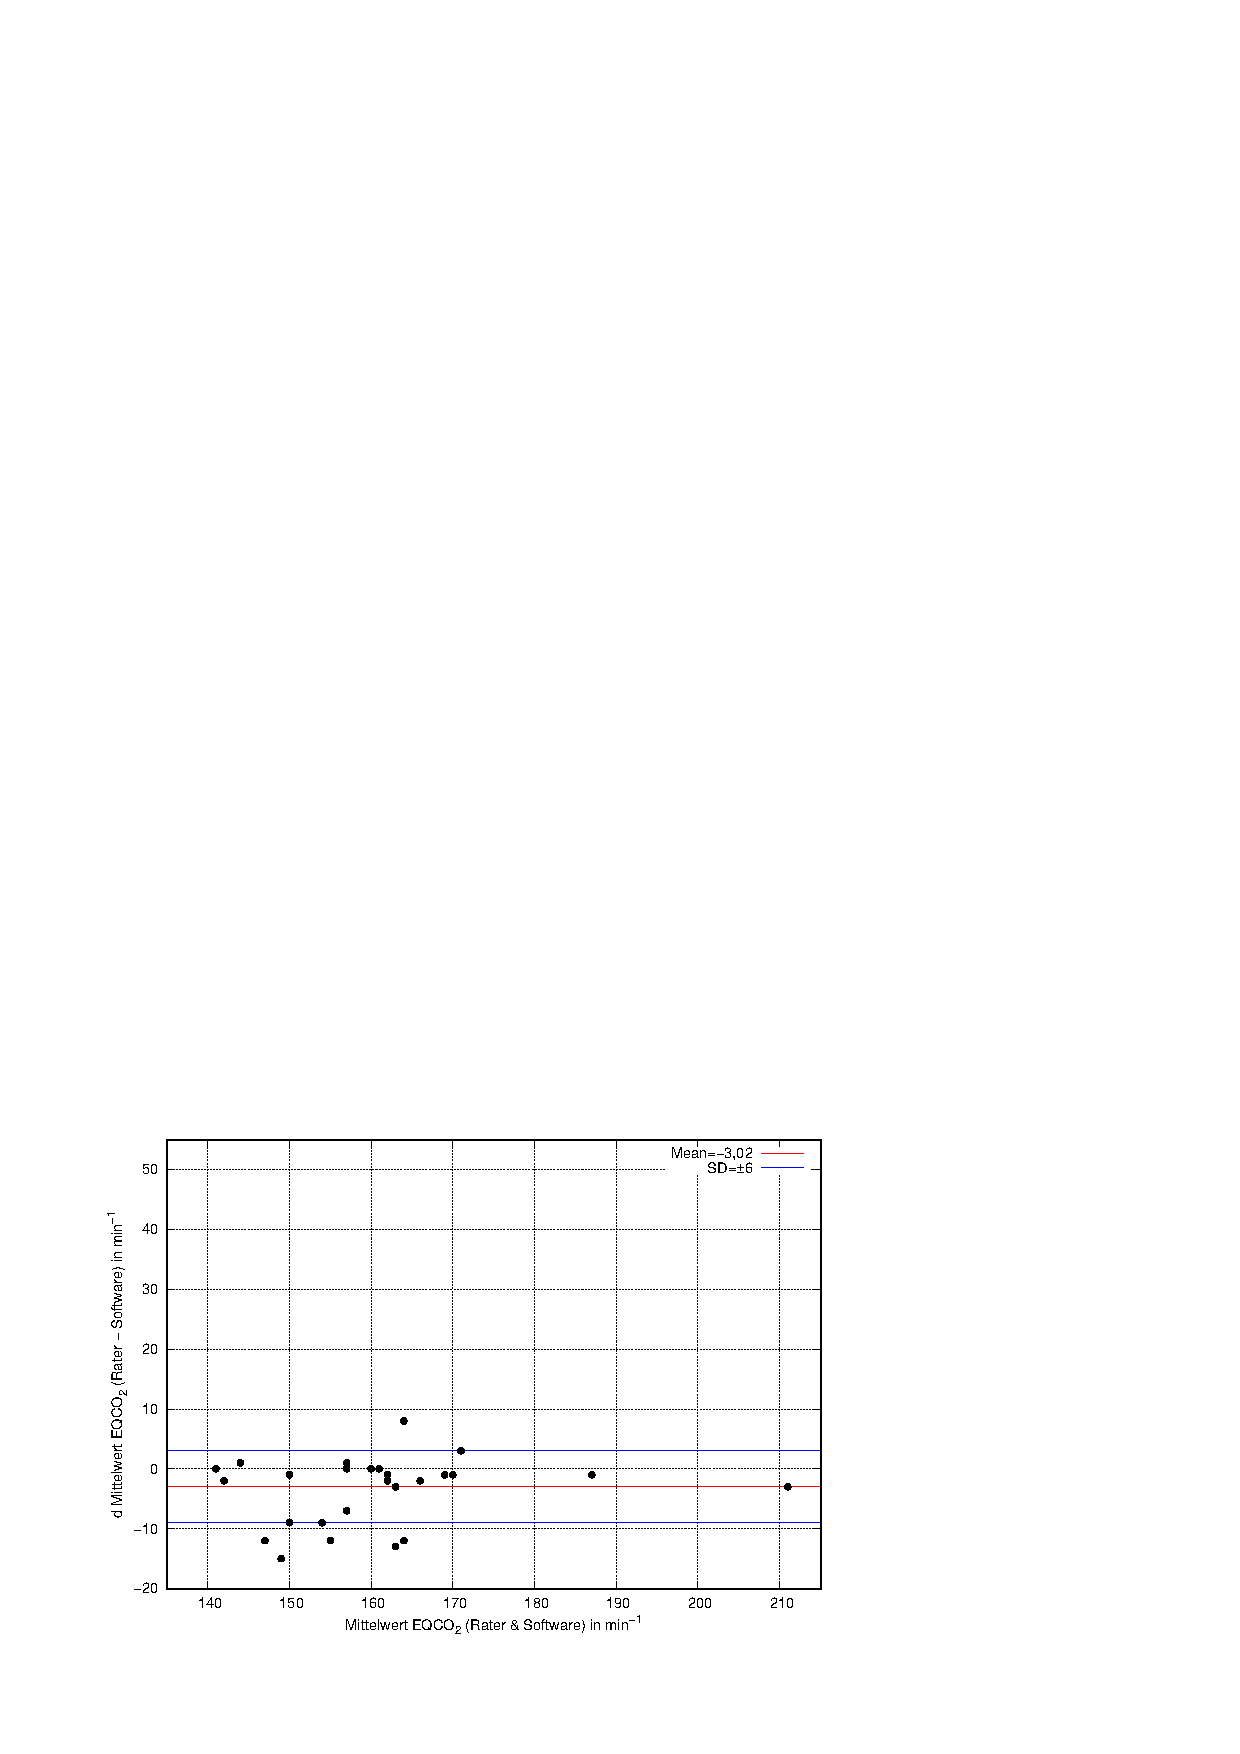
\includegraphics[width=\linewidth]{Bilder/eqco2.png}
		\subcaption{\eqcotwo:\\Anstieg als Folge der Hyperventilation}
	\end{subfigure}
	\hfil
	\begin{subfigure}[t]{0.2\linewidth}
		\centering
		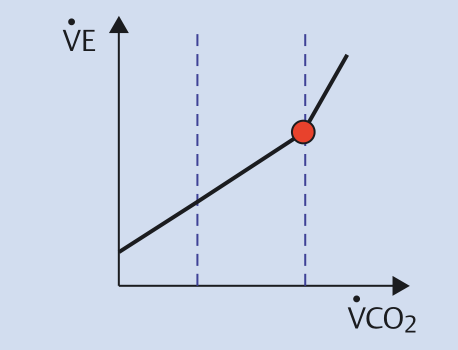
\includegraphics[width=\linewidth]{Bilder/field4.png}
		\subcaption{\ve/\vcotwo:\\überproportionaler Anstieg der \ve{} als Folge der Hyperventilation}
	\end{subfigure}
\end{figure}
\end{column}
\end{columns}
\end{frame}

% -----------------------------------------------------------
% Kapitel 3: Herausforderung & Aufgabenstellung
% -----------------------------------------------------------

\section{Herausforderungen \& Aufgabenstellung}

\begin{frame}
\begin{block}{Unternehmensziele}
	\begin{itemize}
		\item Optimale Methode zur Schwellenbestimmung für optimierten Algorithmus mit Fahrradergometrie erarbeiten
		\item Neue Basis für eine zuverlässigere Definition der Trainingsbereiche erstellen
	\end{itemize}
\end{block}
\begin{block}{Forschungsfragen}
	\begin{enumerate}
		\item Eignet sich der metabolicscan zur Durchführung einer Spiroergometrie?
		\item Mit welcher Methode können die Schwellen optimal bestimmt werden?
		\item Ist eine genauere Bestimmung der VT2 mit den neuen Methoden möglich?
	\end{enumerate}
\end{block}
\end{frame}

% -----------------------------------------------------------
% Kapitel 3: Methoden
% -----------------------------------------------------------
\section{Methode}

\begin{frame}{Versuchsreihe}
\begin{itemize}
	\item Testmessungen mit 28 internen und externen Probanden unter gleichen Bedingungen (räumliche Gegebenheiten, Ernährungszustand etc.)
	\item Probanden: m/w, 19 bis 58 Jahre, Sportler und Nicht-Sportler, Raucher und Nichtraucher
	\item Anamnesegespräch + Ruhe-EKG + Bestimmung der ungefähren Soll-Belastung und des individuellen Belastungsprotokolls mit Rücksicht auf Trainingszustand
	\item Leerlastphase (\SI{2}{\minute}) $\rightarrow$ Ruhestoffwechselmessung $\rightarrow$ Belastungsphase
	\item Belastungsphase: \SI{2}{\minute} (\SI{90}{\second} frei, \SI{30}{\second} messen) $\rightarrow$ Inkrement: \SI{25}{\watt} nach WHO-Schema~(\cite{Trappe.2000})
	\item Speichern der Sensor-Rohdaten in Textdateien
	\item Weiterverarbeitung + Auswertung durch ein MATLAB-Programm
	\item Schwellenbestimmung: manuell durch zwei Rater + algorithmisch
	\item Statistische und methodenkritische Analyse der Ergebnisse
\end{itemize}
\end{frame}

\begin{frame}{Funktionsweise des metabolicscan}
\begin{columns}
\begin{column}{0.5\linewidth}
\begin{itemize}
	\item Modularer Aufbau: Atemmodul mit Flowsensor + Analysemodul mit CO\textsubscript{2}/O\textsubscript{2}-Sensormodul
	\item Atemmodul: Messung der Strömungsgeschwindigkeit der Inspirations- und Exspirationsluft
	\item Berechnung des Strömungsvolumens durch mathematische Integration über die Zeit
	\item Pumpe saugt Luftanteil durch Probenschlauch zum Analysemodul
	\item Analysemodul: CO\textsubscript{2}-Messung durch Infrarotlichtabsorption
	\item Weiterleitung zum galvanischen O\textsubscript{2}-Sensor $\rightarrow$ O\textsubscript{2}-Konzentration ist proportional zu fließendem Strom
\end{itemize}
\end{column}
\begin{column}{0.5\linewidth}
			\begin{figure}[H]
				\centering
				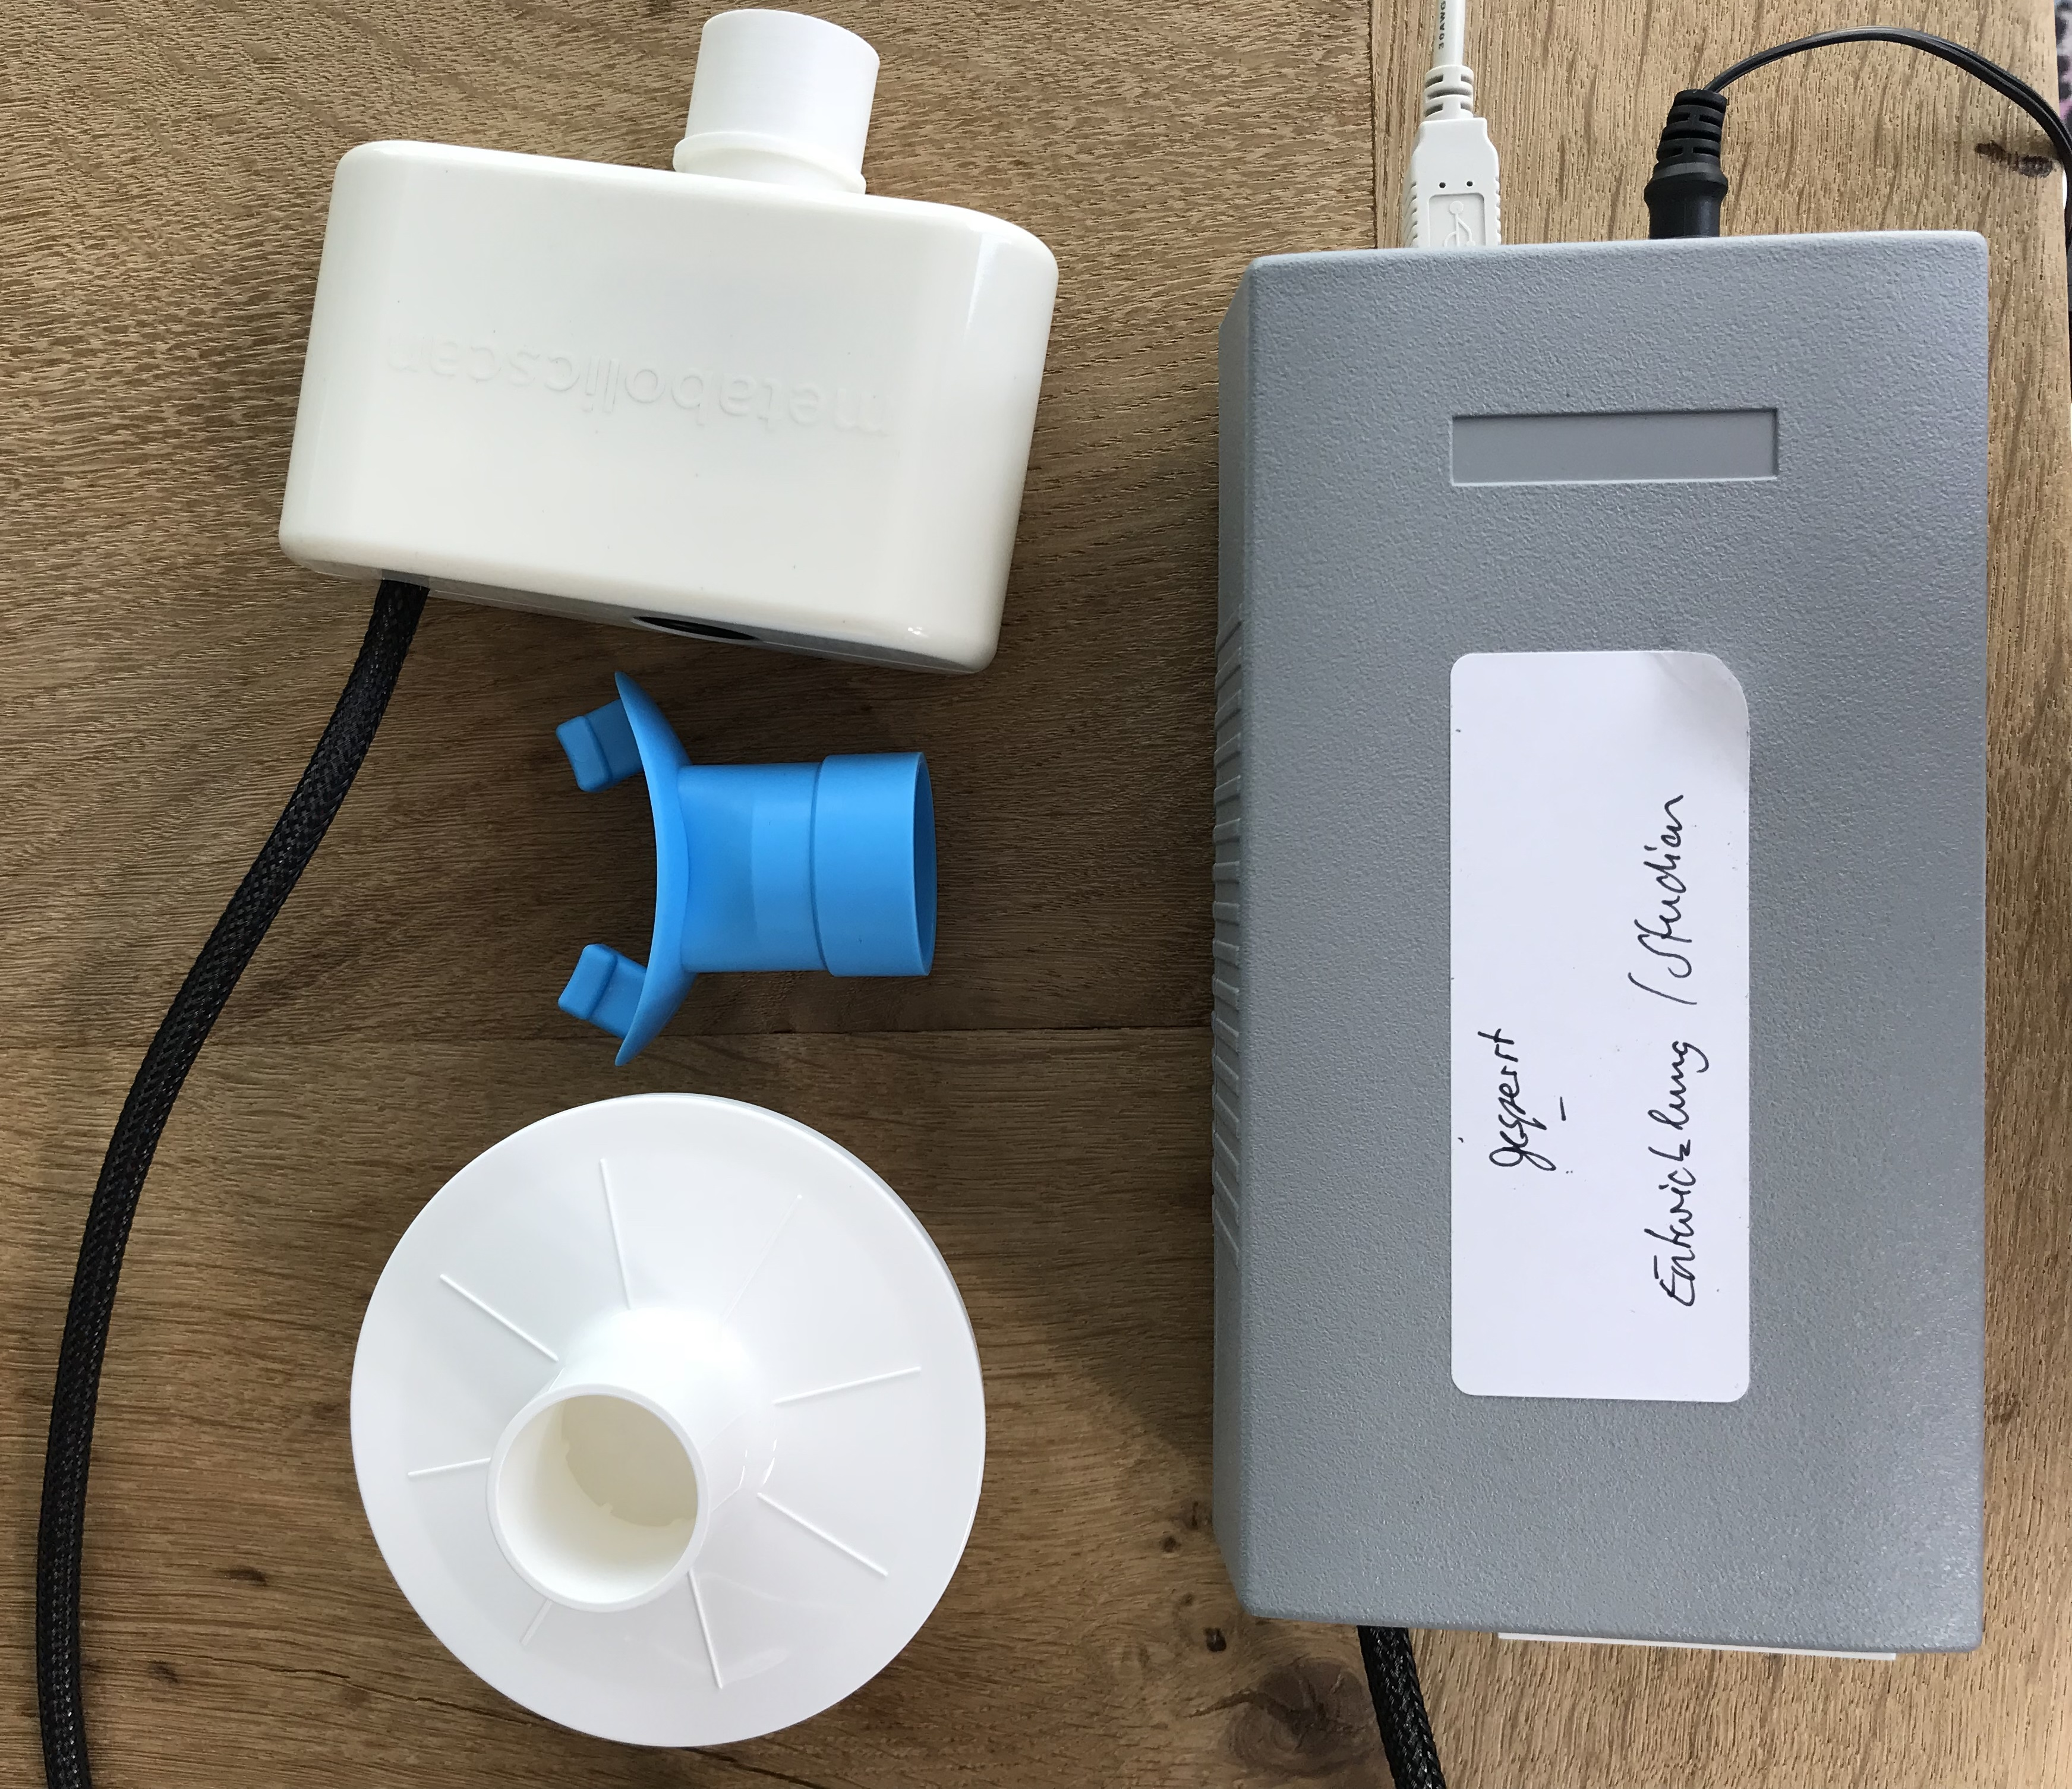
\includegraphics[width=0.8\linewidth]{Bilder/mbs.jpg}
				\caption{metabolicscan: Analysemodul, Atemmodul, Filter und Mundstück}
			\end{figure}
\end{column}
\end{columns}
\end{frame}

% -----------------------------------------------------------
% Kapitel 4: Resultate
% -----------------------------------------------------------
\section{Resultate}

\begin{frame}{"`6-Felder-Grafiken"'}
	\begin{itemize}
		\item Keine Sensor-Störungen oder Gerätefehler während der Messungen
		\item Zwei "`6-Felder-Grafiken"' für jeden Probanden generiert: eine für manuelle Bestimmung, eine mit algorithmischen Schwellenbestimmungen
		\item Vorwiegend bei den VT1-Methoden teilweise nicht-differenzierbare Plots
		\item Differenzen zwischen den einzelnen Ergebnissen der Rater und Software\\$\rightarrow$ statistische Auswertung
	\end{itemize}
	\begin{figure}[H]
		\begin{subfigure}[c]{0.45\linewidth}
			\centering
			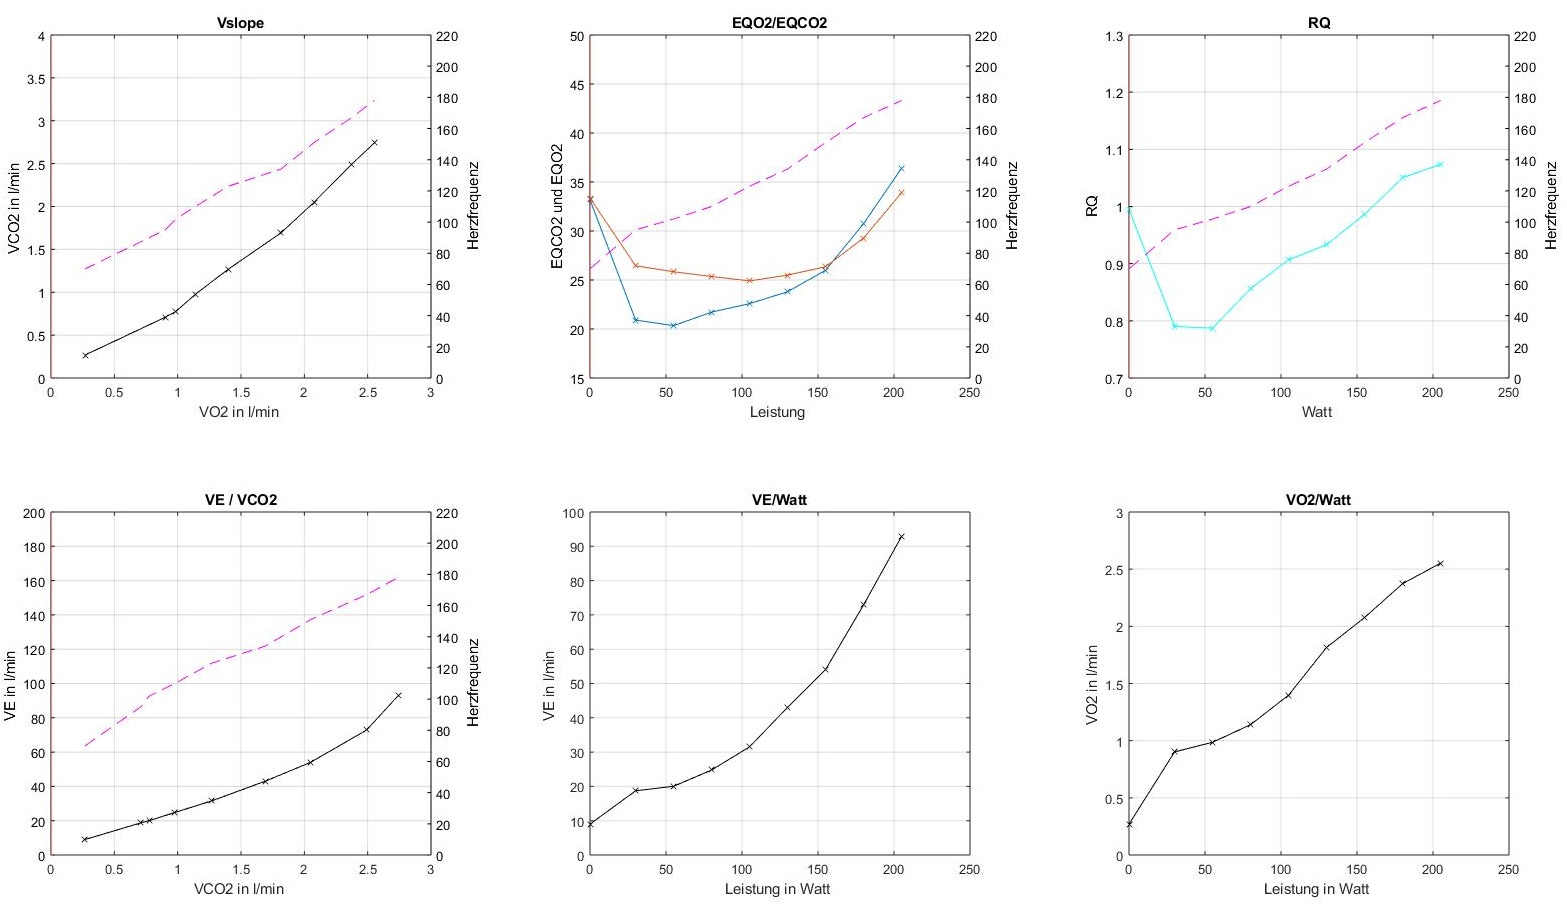
\includegraphics[width=\linewidth]{Bilder/plot_6w.jpg}
			\subcaption{Blankoplot}
		\end{subfigure}
		\hfil
		\begin{subfigure}[c]{0.45\linewidth}
			\centering
			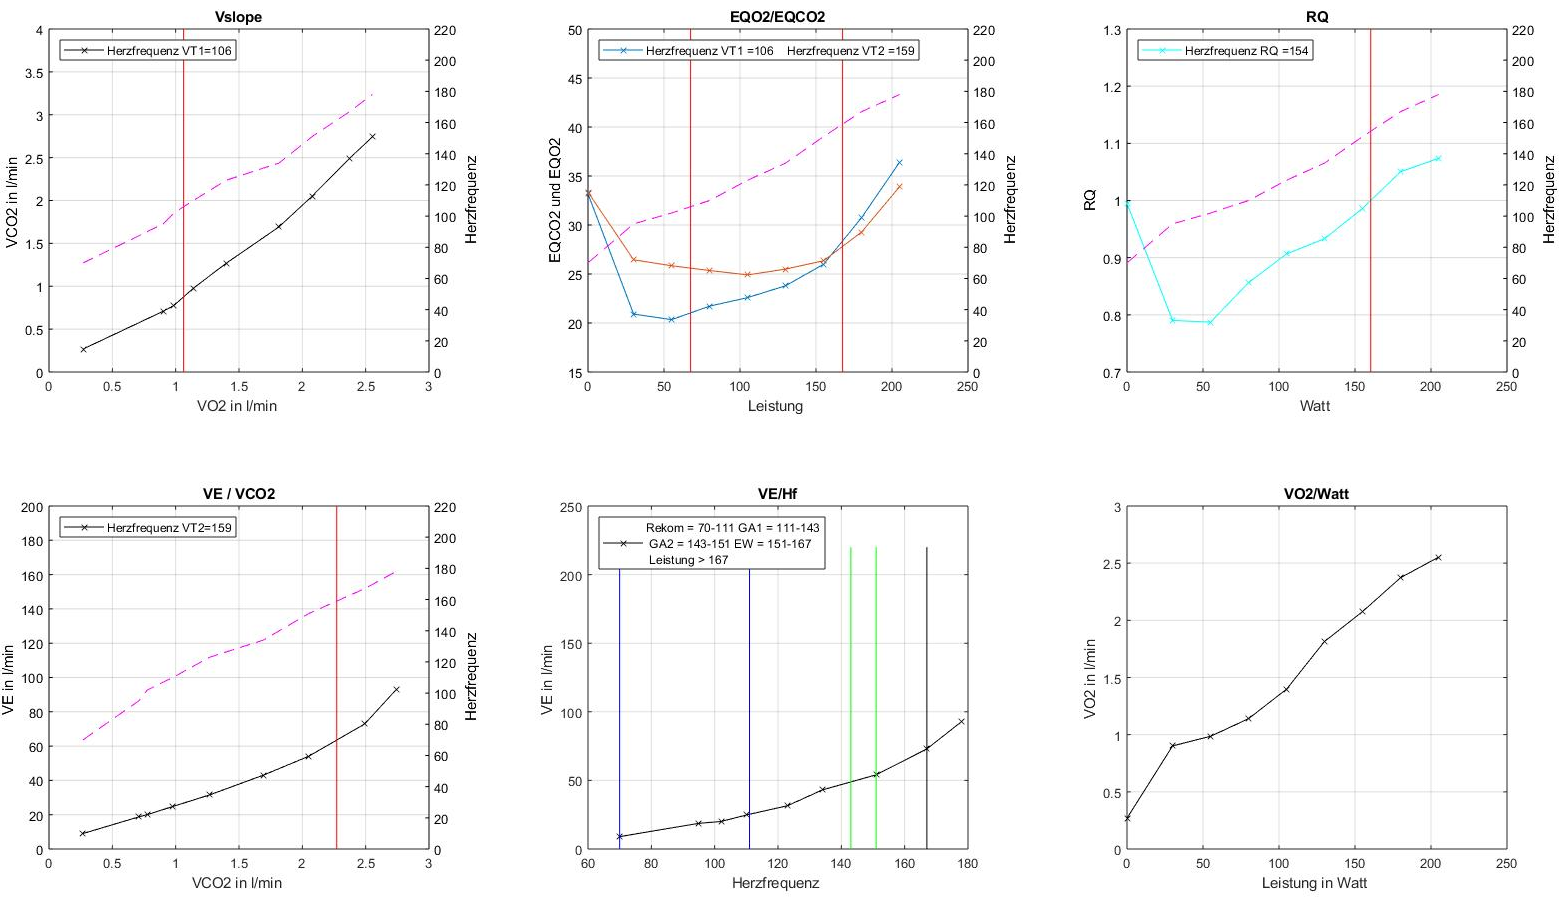
\includegraphics[width=\linewidth]{Bilder/auto_6.png}
			\subcaption{Plot mit algorithmisch bestimmten Schwellen}
		\end{subfigure}
	\end{figure}
\end{frame}

\begin{frame}{Beispielplot 1}
	\begin{figure}[H]
		\centering
			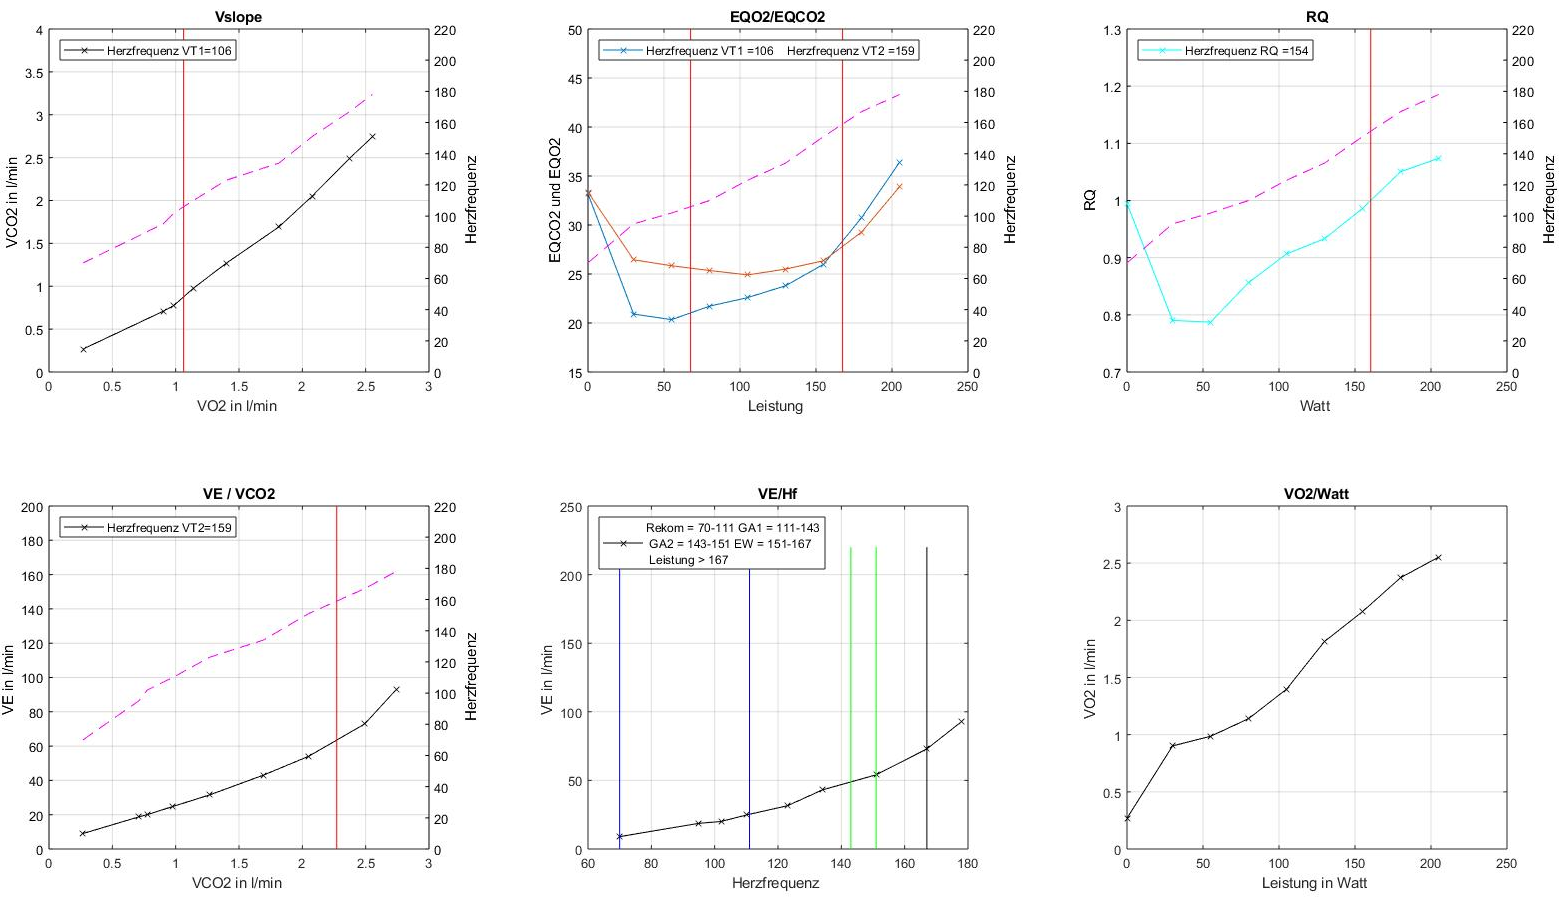
\includegraphics[width=0.85\linewidth]{Bilder/auto_6.png}
			\caption{Beispielplot der Probandin 6w}
	\end{figure}
\end{frame}

\begin{frame}{Beispielplot 2}
	\begin{figure}[H]
		\centering
			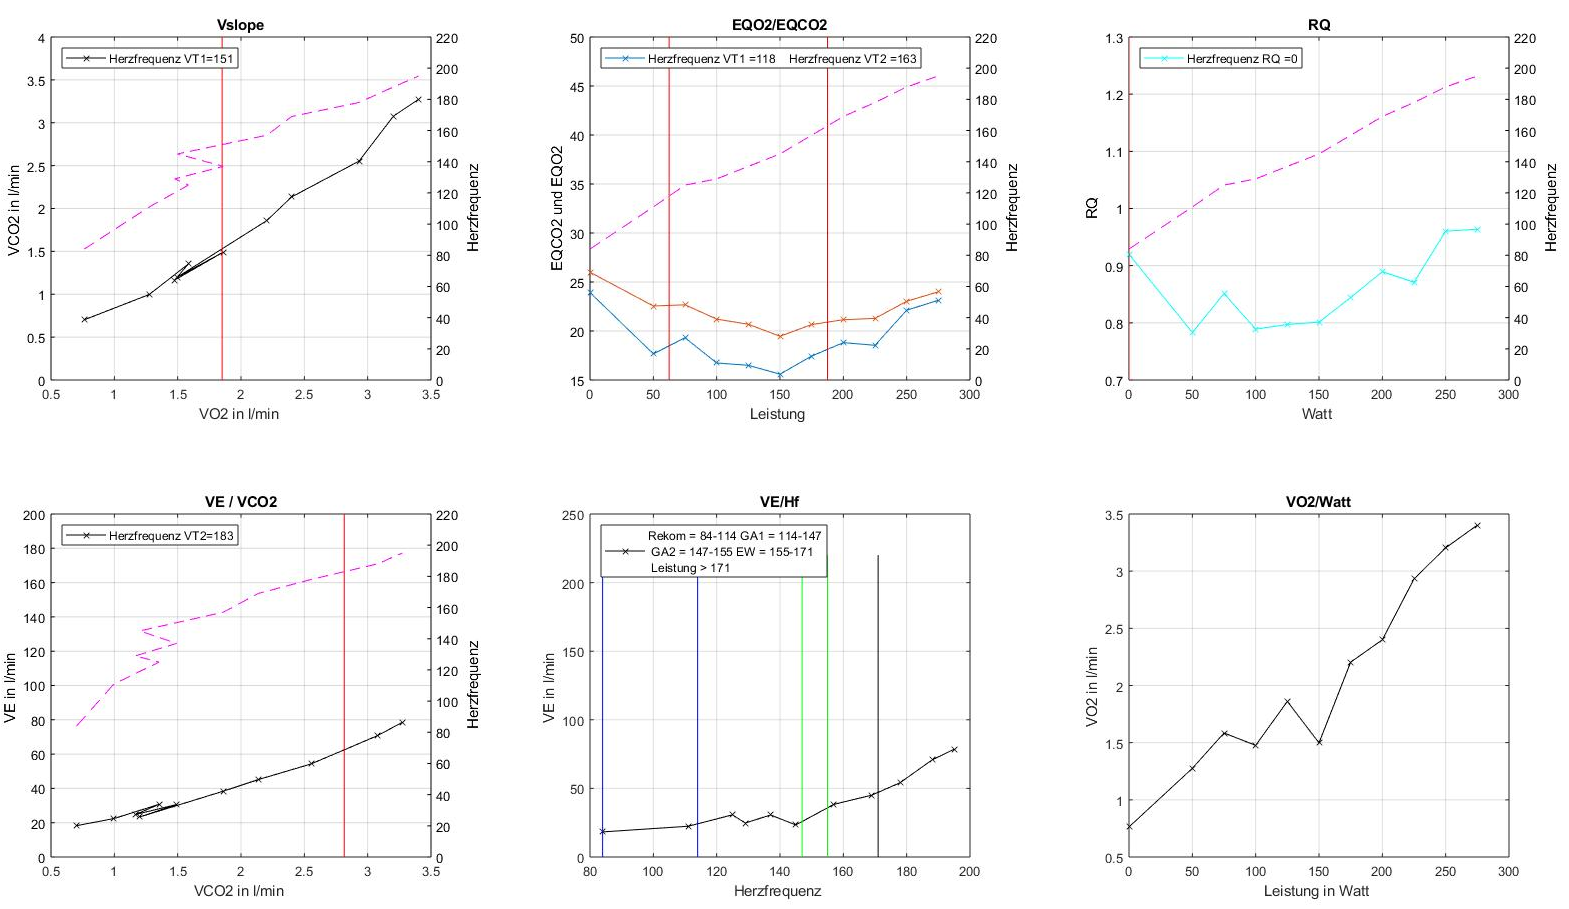
\includegraphics[width=0.85\linewidth]{Bilder/auto_21.png}
			\caption{Beispielplot des Probanden 21m}
	\end{figure}
\end{frame}

\begin{frame}[fragile]{VT1-Ergebnisse}
\begin{columns}
	\begin{column}{0.5\linewidth}
		\begin{figure}
			\begin{subfigure}{0.9\linewidth}
				\centering
				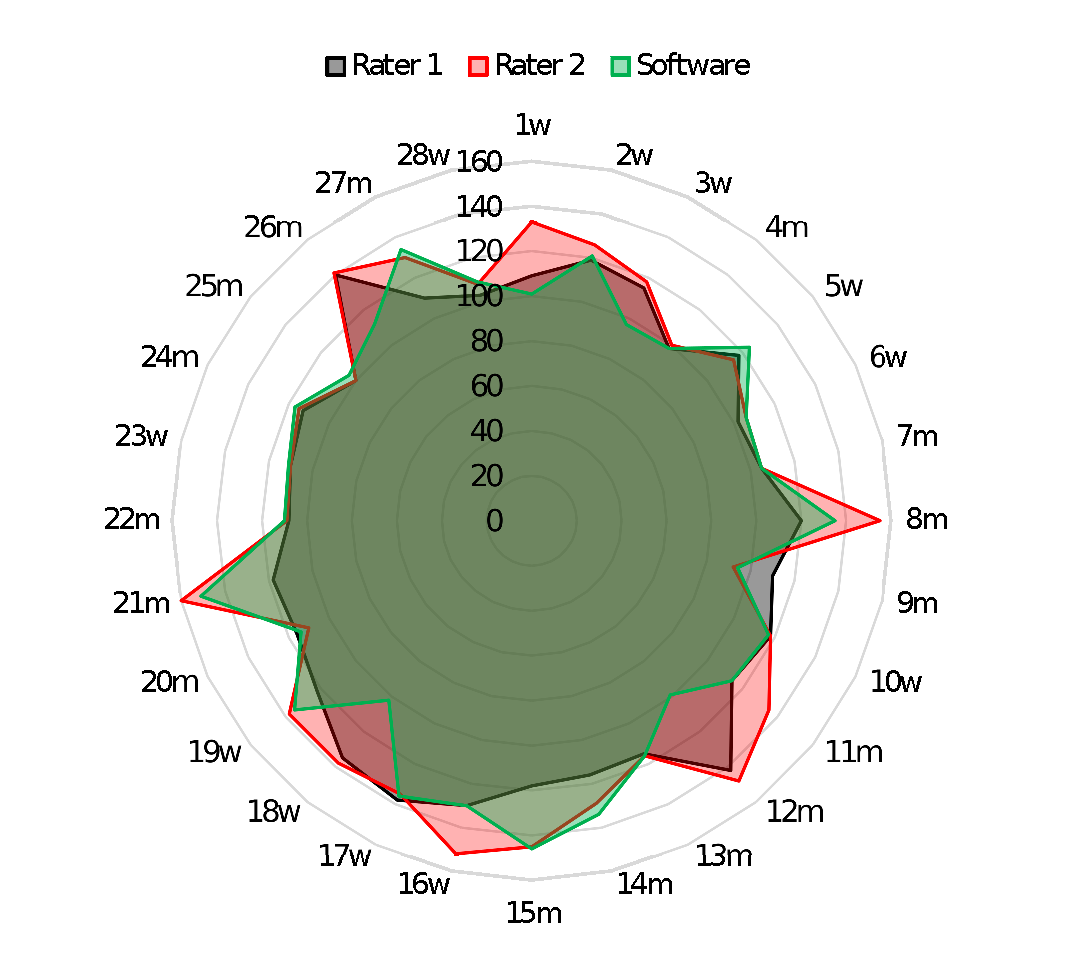
\includegraphics[width=0.6\linewidth]{Bilder/v-slope_net.eps}
			\end{subfigure}
			\begin{subfigure}{0.9\linewidth}
				\centering
				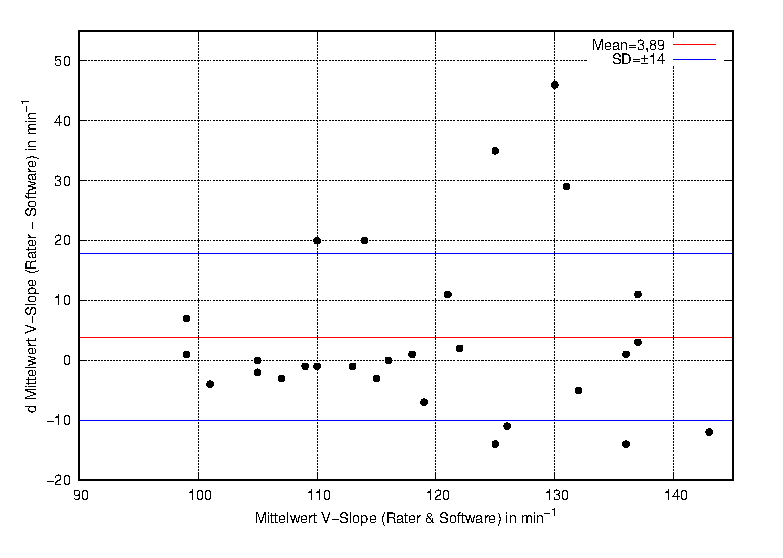
\includegraphics[width=0.82\linewidth]{Bilder/vslope.eps}
			\end{subfigure}	
			\caption{V-Slope}	
		\end{figure}
	\end{column}
	\begin{column}{0.5\linewidth}
		\begin{figure}
			\begin{subfigure}{0.9\linewidth}
				\centering
				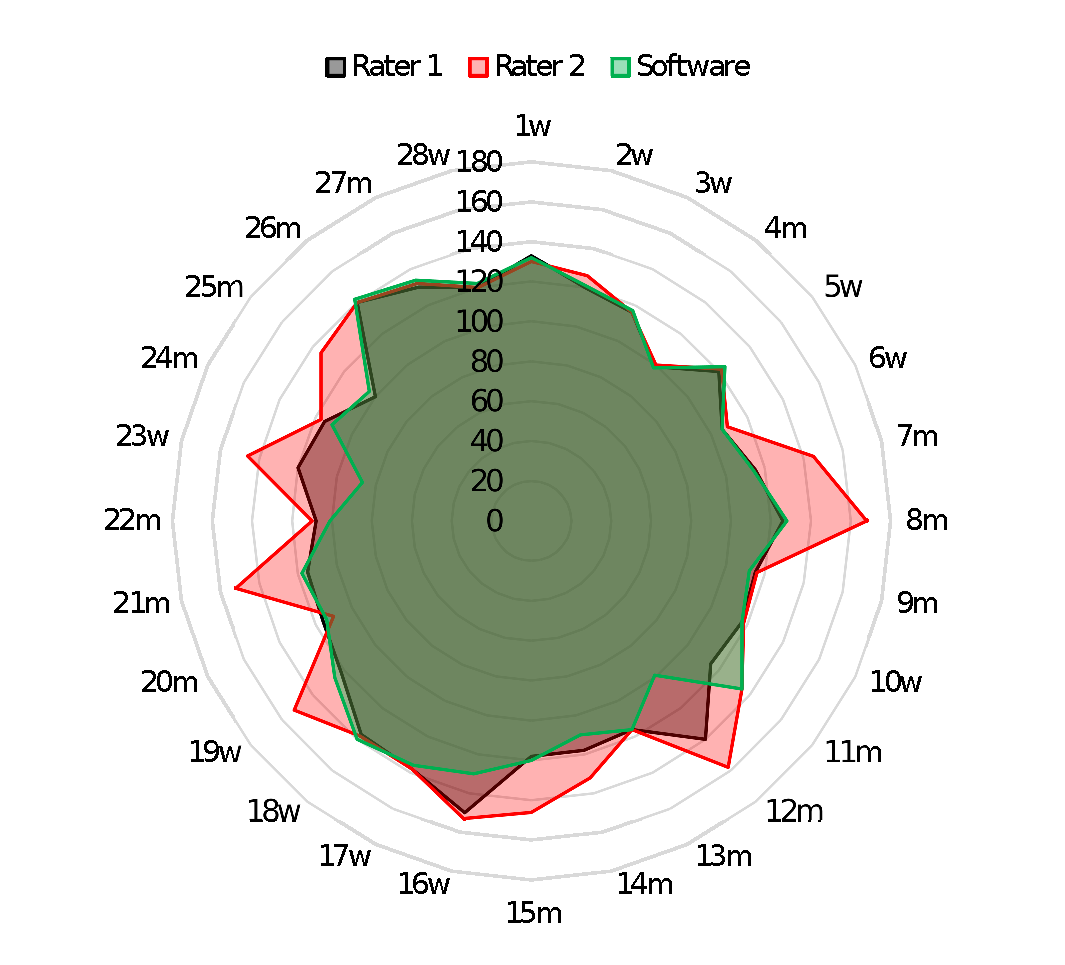
\includegraphics[width=0.6\linewidth]{Bilder/eqo2_net.eps}
			\end{subfigure}
			\begin{subfigure}{0.9\linewidth}
				\centering
				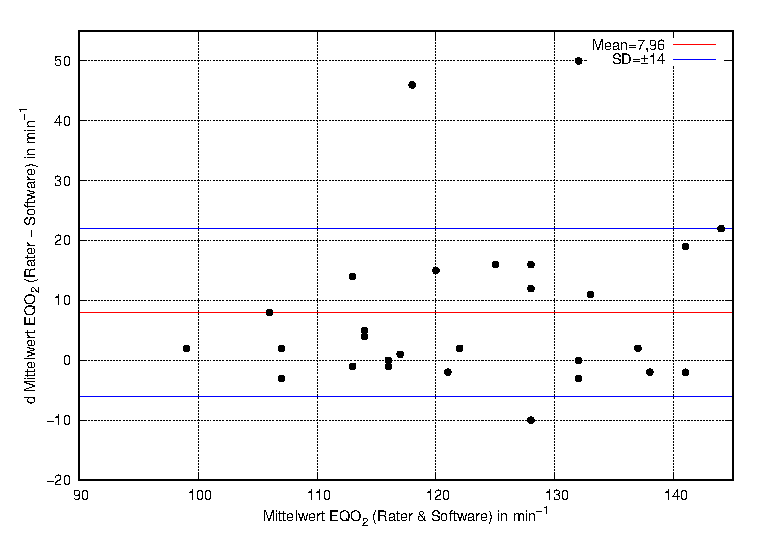
\includegraphics[width=0.82\linewidth]{Bilder/eqo2.eps}
			\end{subfigure}	
			\caption{\eqotwo}
		\end{figure}
	\end{column}
\end{columns}
\end{frame}

\begin{frame}[fragile]{VT2-Ergebnisse}
\begin{columns}
	\begin{column}{0.5\linewidth}
		\begin{figure}
			\begin{subfigure}{0.9\linewidth}
				\centering
				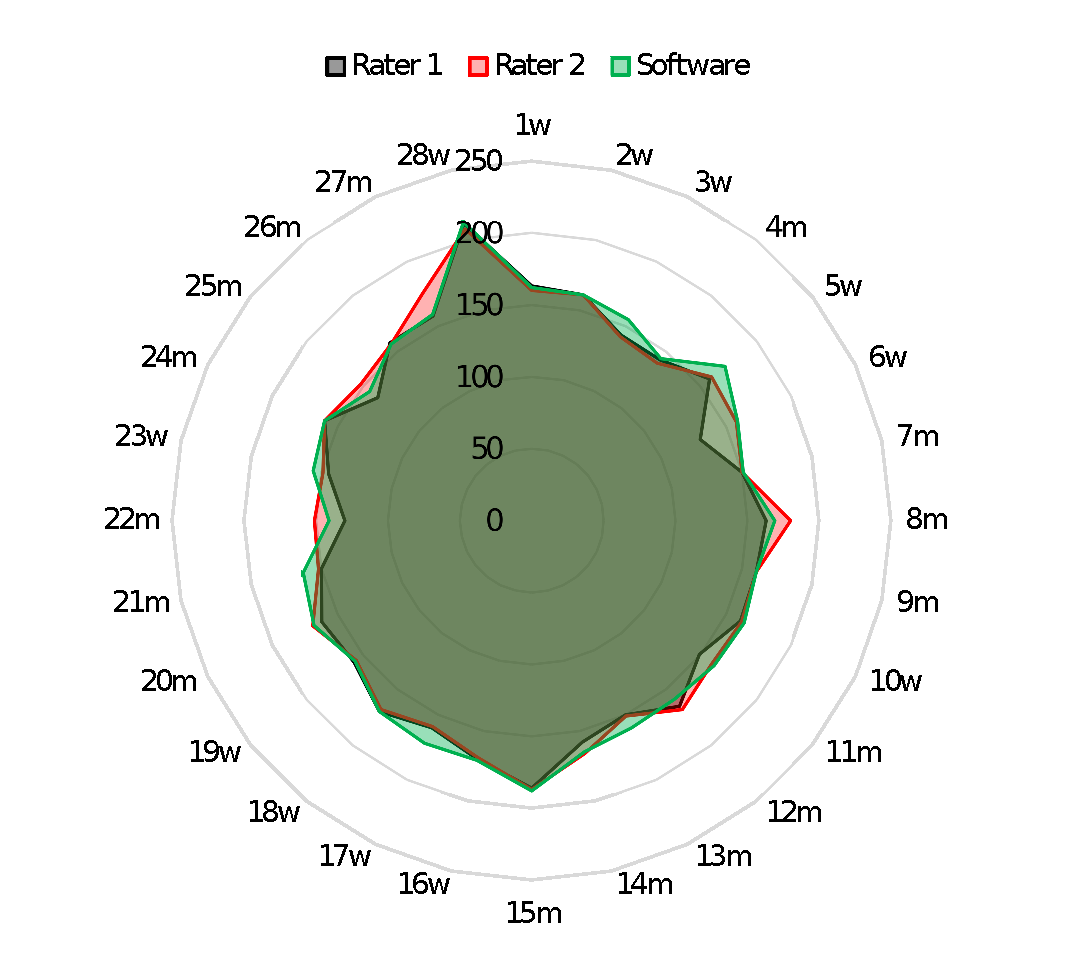
\includegraphics[width=0.6\linewidth]{Bilder/eqco2_net.eps}
			\end{subfigure}
			\begin{subfigure}{0.9\linewidth}
				\centering
				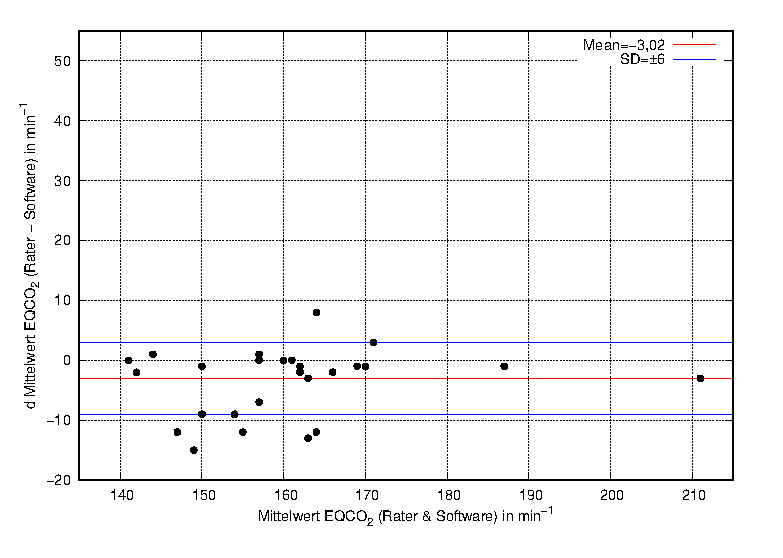
\includegraphics[width=0.82\linewidth]{Bilder/eqco2.eps}
			\end{subfigure}	
		\caption{\eqcotwo}	
		\end{figure}
	\end{column}
	\begin{column}{0.5\linewidth}
		\begin{figure}
			\begin{subfigure}{0.9\linewidth}
				\centering
				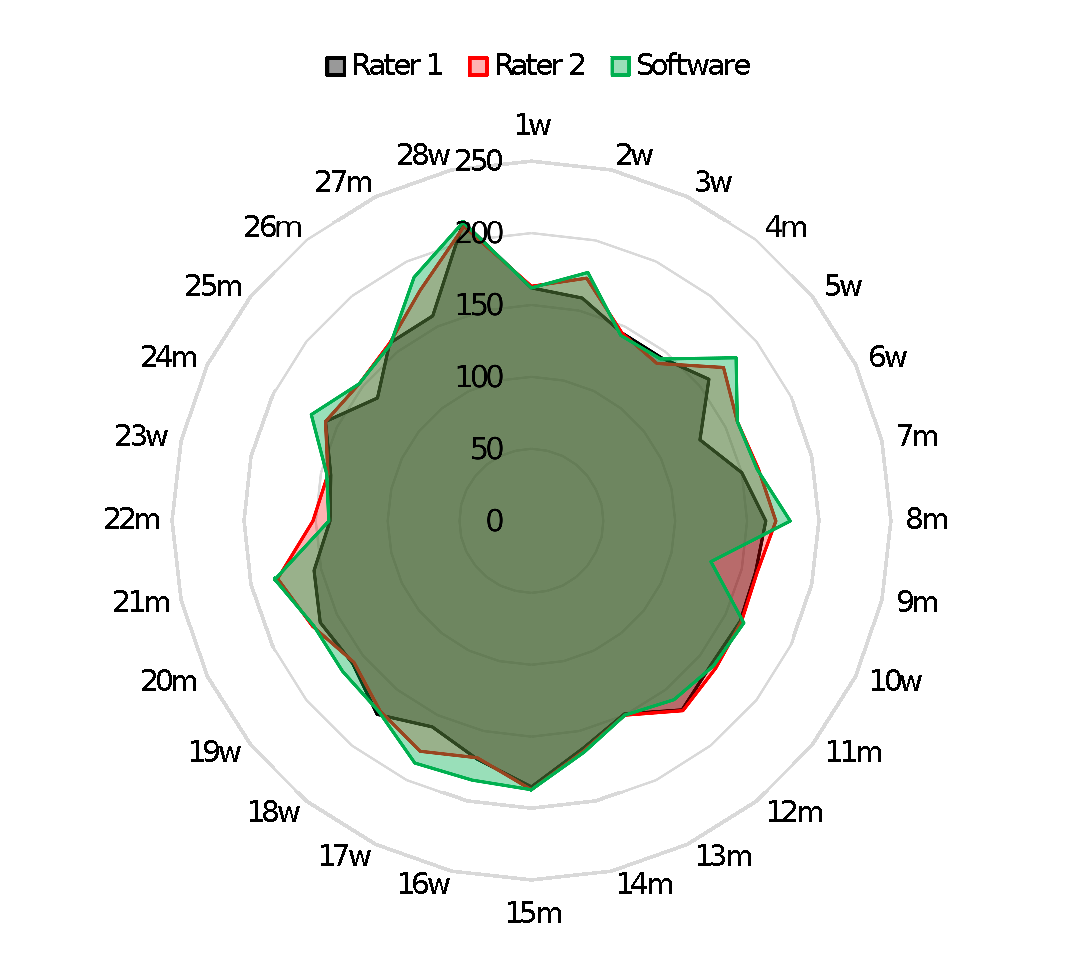
\includegraphics[width=0.6\linewidth]{Bilder/vevco2_net.eps}
			\end{subfigure}
			\begin{subfigure}{0.9\linewidth}
				\centering
				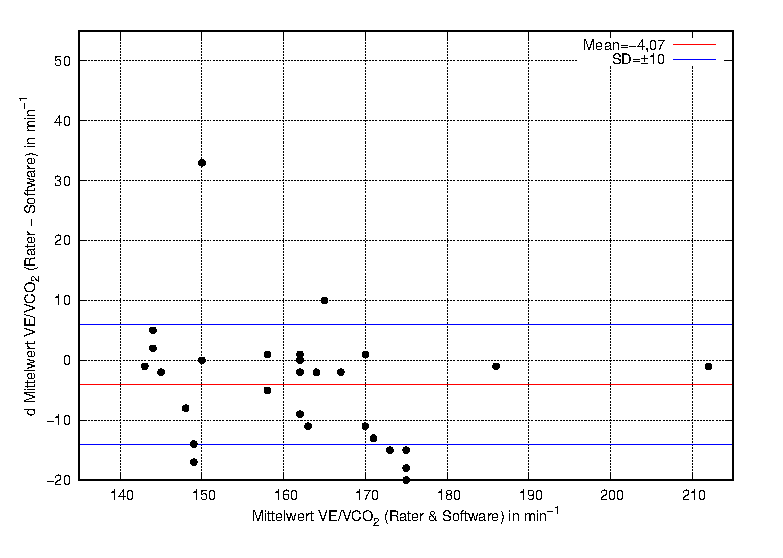
\includegraphics[width=0.82\linewidth]{Bilder/vevco2.eps}
			\end{subfigure}	
		\caption{\ve/\vcotwo}
		\end{figure}
	\end{column}
\end{columns}
\end{frame}

% -----------------------------------------------------------
% Kapitel 5: Diskussion
% -----------------------------------------------------------
\section{Diskussion}

\begin{frame}{Evaluation der Tests}
\begin{itemize}
	\item VT1-Bestimmung erschwert durch kritische Plots erschwert
	\item Analyse der Felder 5 und 6: Plausibilitätsprüfung des Verlaufs der \ve{} bzw. der \vcotwo{} zur W\\$\rightarrow$ Annahme: idealerweise lineare Zunahme~(\cite{Ruehle.2012})
	\item Erkenntnis: Schwankungen zurückzuführen auf Fehler im Algorithmus
	\item Für alle Testmessungen konnten charakteristische Graphen generiert werden
	\item Alle erhobenen Messwerte lagen innerhalb der maximal zulässigen Grenzwerte der Sensoren
\end{itemize}
\end{frame}

\begin{frame}{Evaluation der Methoden}
\begin{columns}
\begin{column}{0.5\linewidth}
\begin{figure}[H]
	\centering
	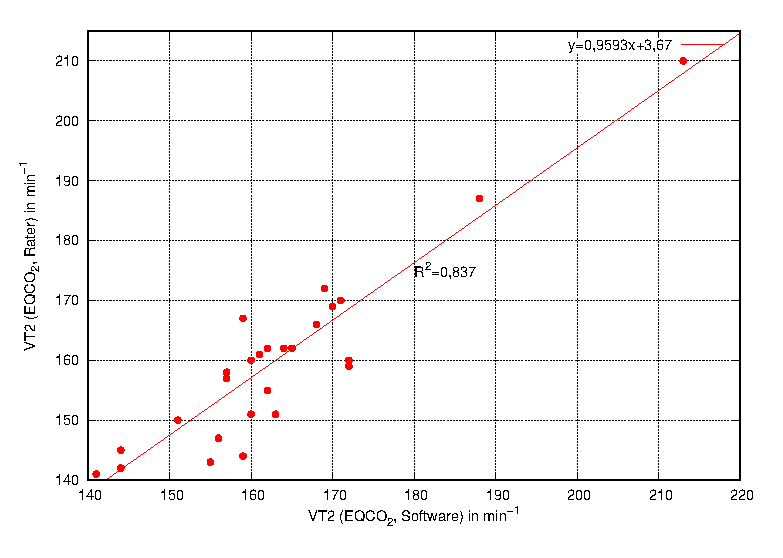
\includegraphics[width=\linewidth]{Bilder/korr_eqco2.eps}
	\caption{Regressionsanalyse der \eqcotwo-Ergebnisse}
\end{figure}
\end{column}
\begin{column}{0.5\linewidth}
	\eqcotwo{} ist die Methode mit den geringsten Abweichungen $\rightarrow$ optimale Methode\\
	\vspace{3ex}
	Korrelationskoeffizient $r = 0,912$\\
	\vspace{3ex}
	\ve/\vcotwo{} als geeignete Referenzmethode mit $r = 0,816$
\end{column}
\end{columns}
\end{frame}

\begin{frame}{Evaluation der Methoden}
\begin{itemize}
	\item V-Slope-Plots häufig nicht differenzierbar $\rightarrow$ viele Differenzen $\rightarrow$ $r = 0,526$
	\item Schwankungen der \eqotwo-Kurve $\rightarrow$ häufiger große Differenzen $\rightarrow$: $r = 0,464$
	\item Mit einem Modell nach W. Kindermann ist die Trainingszonendefinition nur von VT2 abhängig (\cite{Kindermann.2004})\\$\rightarrow$ VT1 zum Erreichen des Zieles nicht zwingend erforderlich
	\item Mit RQ=1-Methode 9 von 28 Tests nicht auswertbar; bei auswertbaren Plots: häufig hohe Differenzen zu anderen Methoden
	\item Vergleich mit HUNT 3: 15 von 28 Ergebnissen befinden sich innerhalb des geschlechts- und altersspezifischen Durchschnitts\\$\rightarrow$ 12 Ergebnisse eine Stufe niedriger (plausibel, da muskulärer Wirkungsgrad sowie \votwo{} auf Laufband höher und Schwelle später erreicht~(\cite{Kroidl.2015}))
\end{itemize}
\end{frame}

\begin{frame}{Fazit \& Ausblick}
\begin{itemize}
	\item Mit \eqcotwo{} wurde eine genauere Methode zur VT2-Bestimmung erarbeitet
	\item Trainingszonen sind nach dem Modell von Kindermann damit definierbar
	\item Gleitende Mittelung als evtl. Alternative zur Mittelung der Messwerte interessant
	\item Alternativen zum Mundstück könnten Atmung des Probanden optimieren/erleichtern\\$\rightarrow$ Reduktion von Messfehlern
	\item Einige Einflussfaktoren sind bei der Durchführung zu beachten: probandenbedingt, anwenderbedingt, umweltbedingt\\$\rightarrow$ Produkt- und Konzept-Schulungen durch cardioscan Academy sind wichtig
\end{itemize}
\end{frame}

\begin{frame}
\begin{center}
	\large{\textbf{Vielen Dank für Ihre Aufmerksamkeit!}}
\end{center}
\end{frame}

% -----------------------------------------------------------
% Kapitel 6: Literatur
% -----------------------------------------------------------
\section{Literatur}

\begin{frame}
\begin{columns}
\begin{column}{0.9\linewidth}
\nocite{*}
\printbibliography[heading=none]
\end{column}
\end{columns}
\end{frame}

\end{document}